
\vspace{-1em}
\begin{tcolorbox}[width=\textwidth,
    colframe=sapphire,
    colback=white,
    arc=24pt,
    boxrule=5pt,
    boxsep=0.5em]


    \begin{minipage}{\textwidth}
        \centering
        \fontsizesection
        \textbf{Takeaway 1: Temporal Subsampling Attenuates Small-Scale Features}
    \end{minipage}
    \vspace{1em}

    \begin{minipage}{\textwidth}
        \centering
        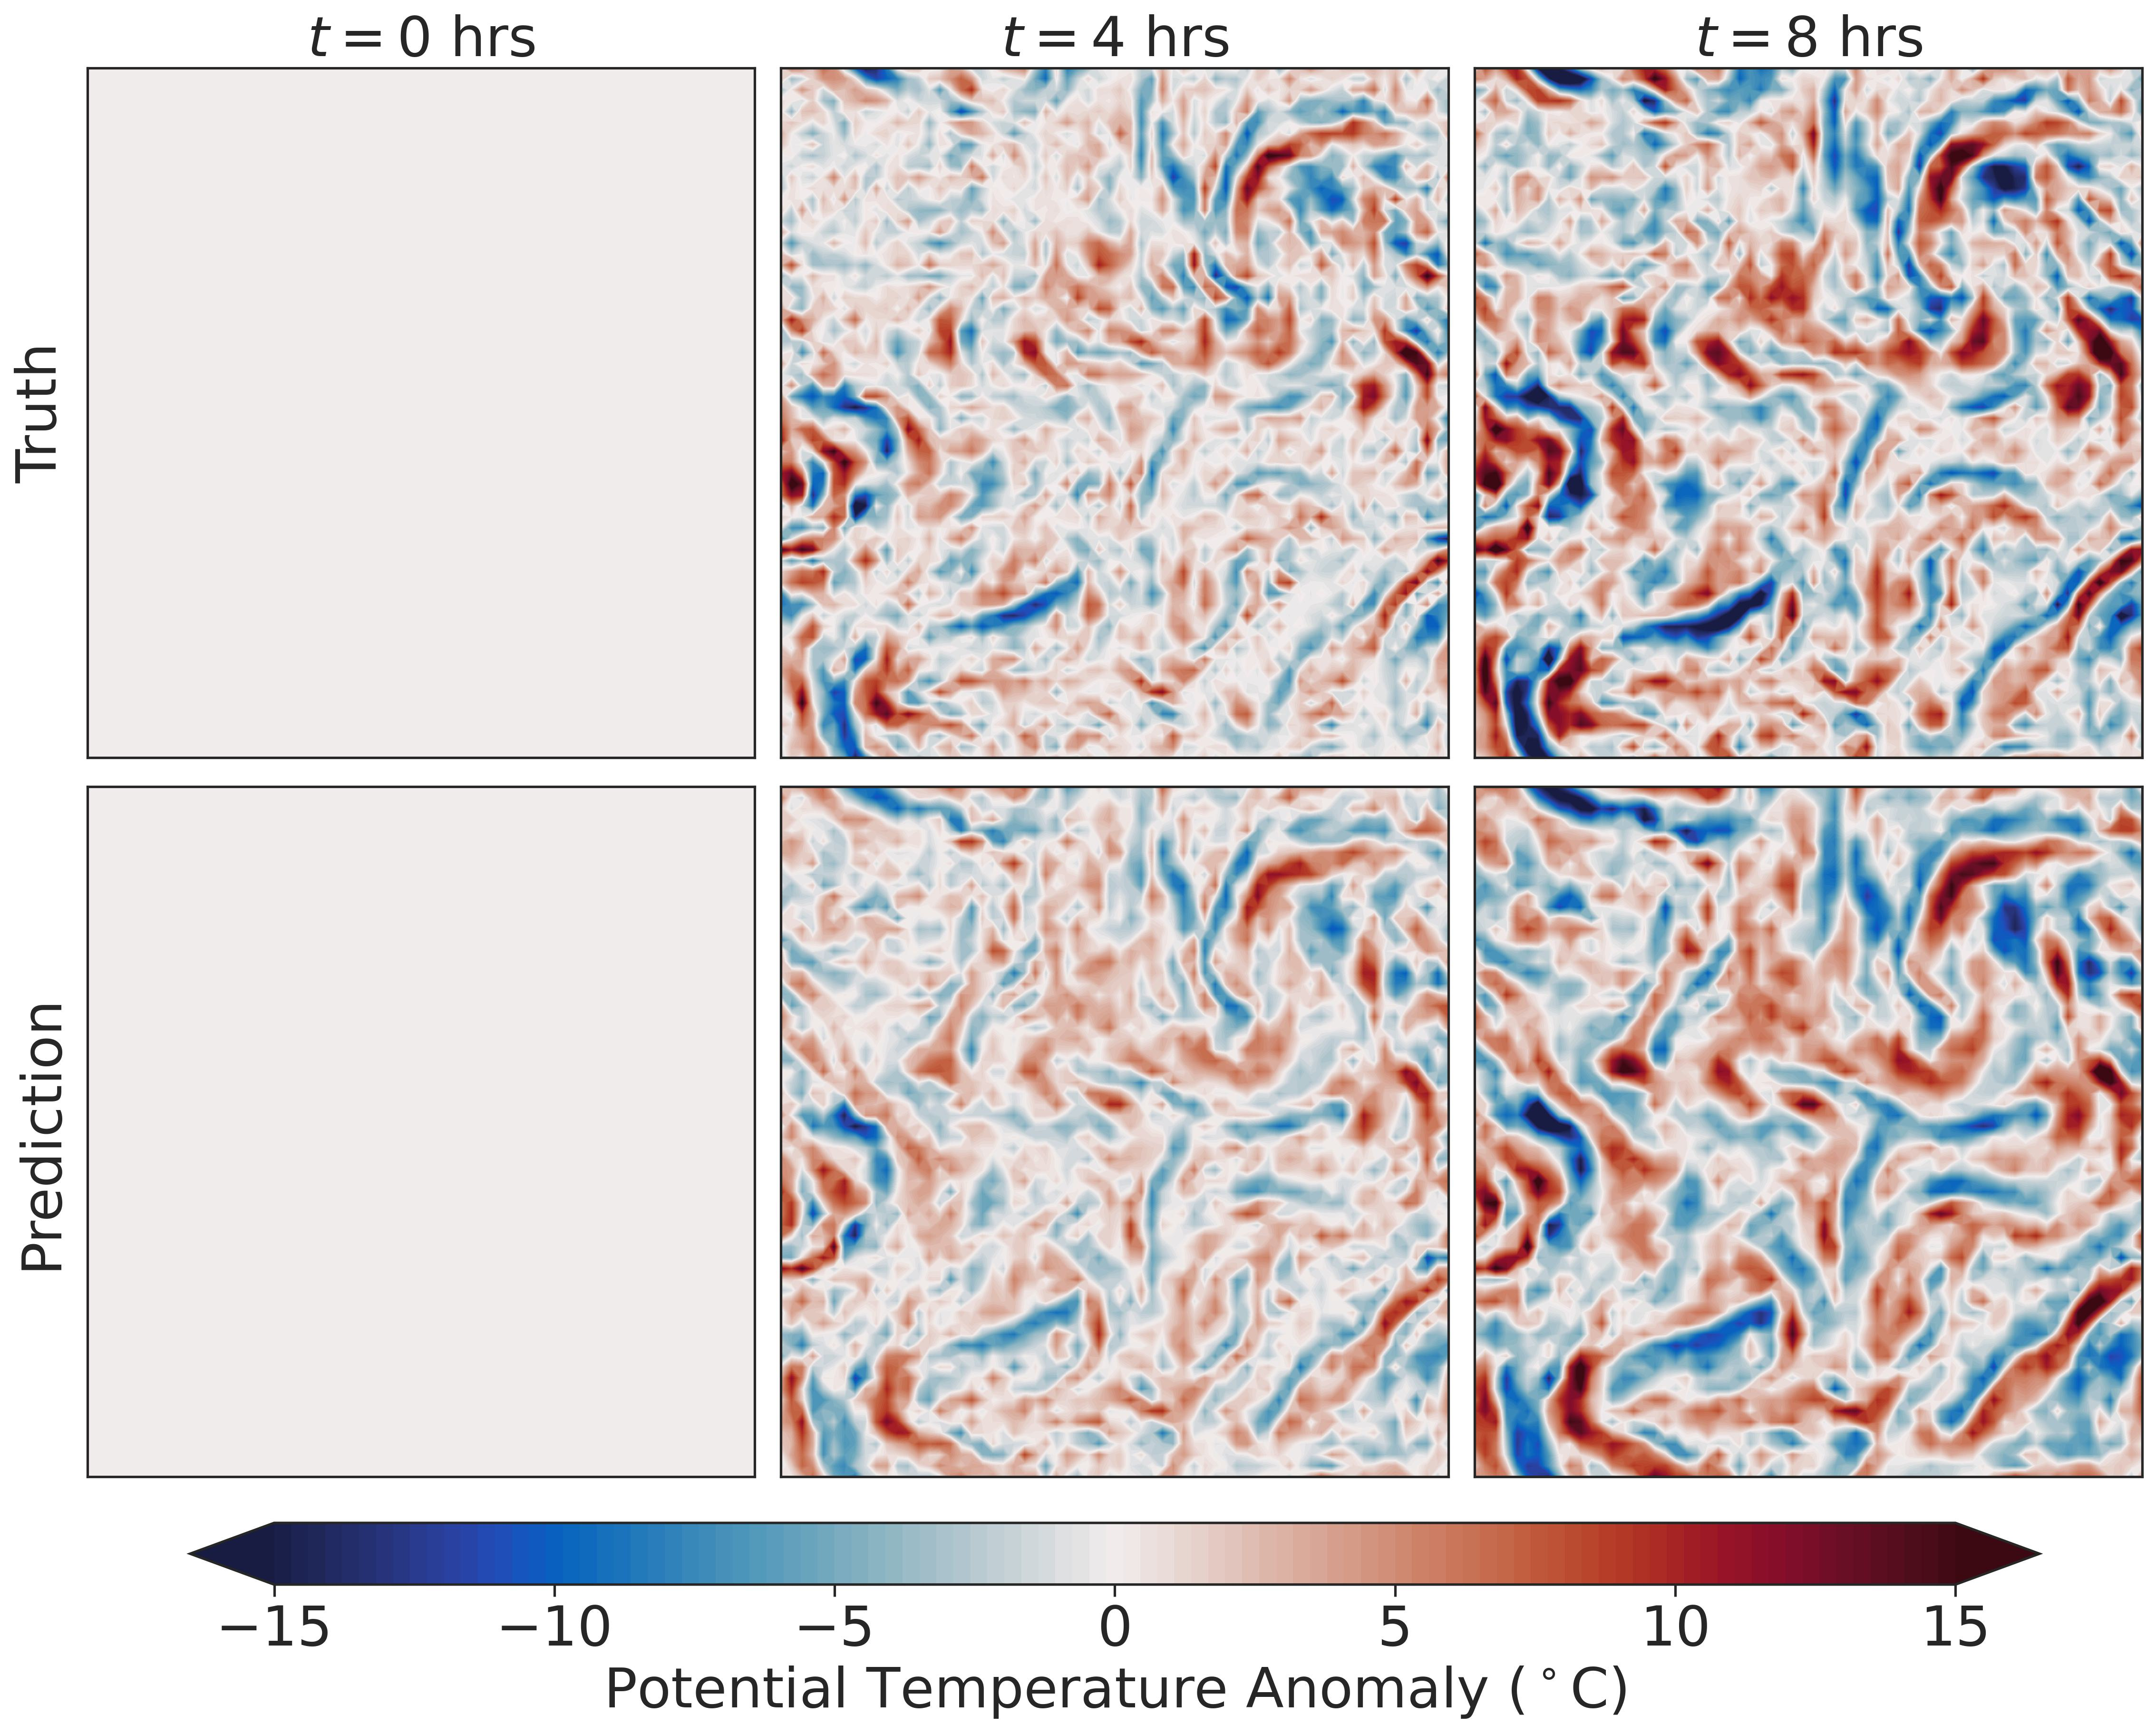
\includegraphics[width=.65\textwidth]{../../figures/nvar-diff-4800dt-nice.jpg}
        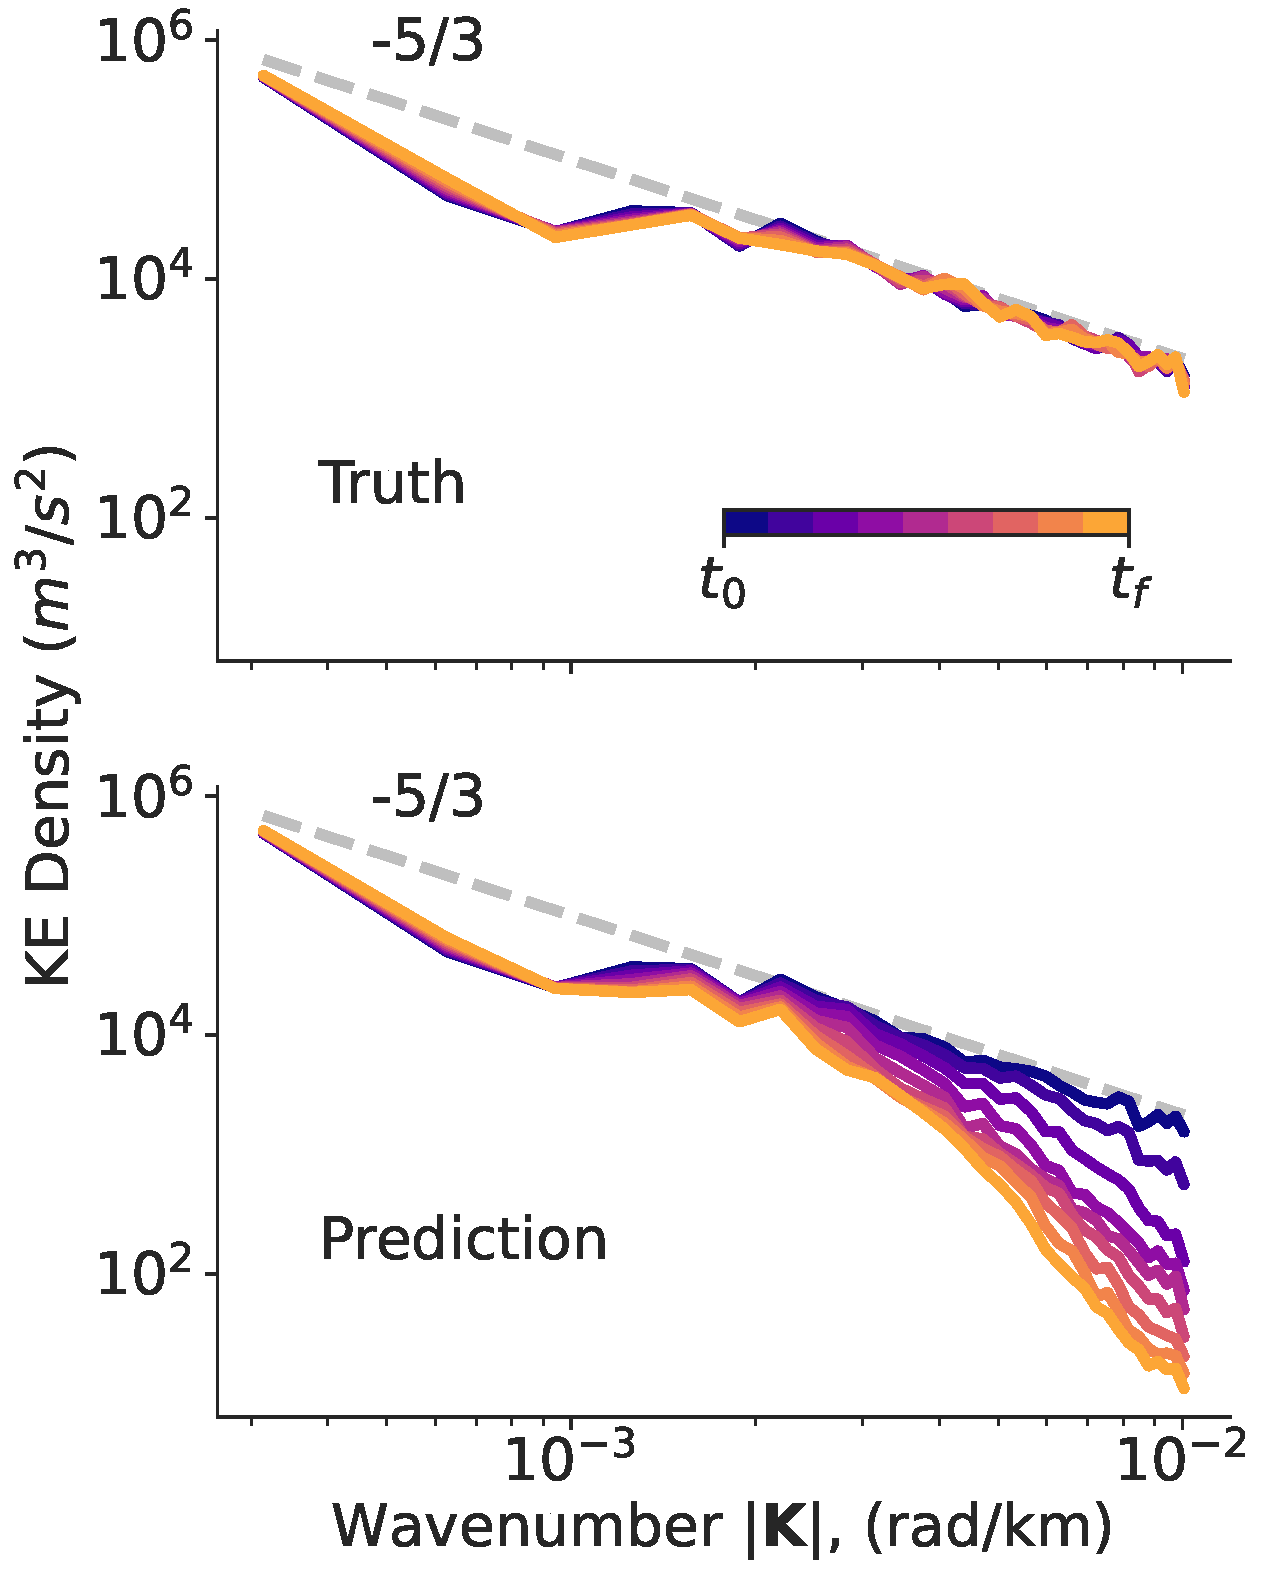
\includegraphics[width=.34\textwidth,trim={0, -2em, 0, 0}, clip]{
        ../../figures/spectrum_4800dt_nice.pdf}
    \end{minipage}

    \vspace{1.5em}
    \begin{minipage}{\textwidth}
        \begin{itemize}
            \item Prediction shows good qualitative resemblance of flow,
                despite\\simplistic NVAR setup
            \item Subsampling removes small scale features, resembling
                CFL-type barrier
            \item Many ML emulators use subsampled reanalysis output for
                training. This subsampling will contribute to a reduced
                ``effective'' resolution.
        \end{itemize}
    \end{minipage}
\end{tcolorbox}


\vspace{2em}
\begin{tcolorbox}[width=\textwidth,
    colframe=sapphire,
    colback=white,
    arc=24pt,
    boxrule=5pt,
    boxsep=0.5em]


   \begin{minipage}{\textwidth}
       \centering
       \fontsizesection
       \textbf{Takeaway 2: Memory Improves Prediction Skill}
   \end{minipage}
   \vspace{1em}

    \begin{minipage}{\textwidth}
        \centering
        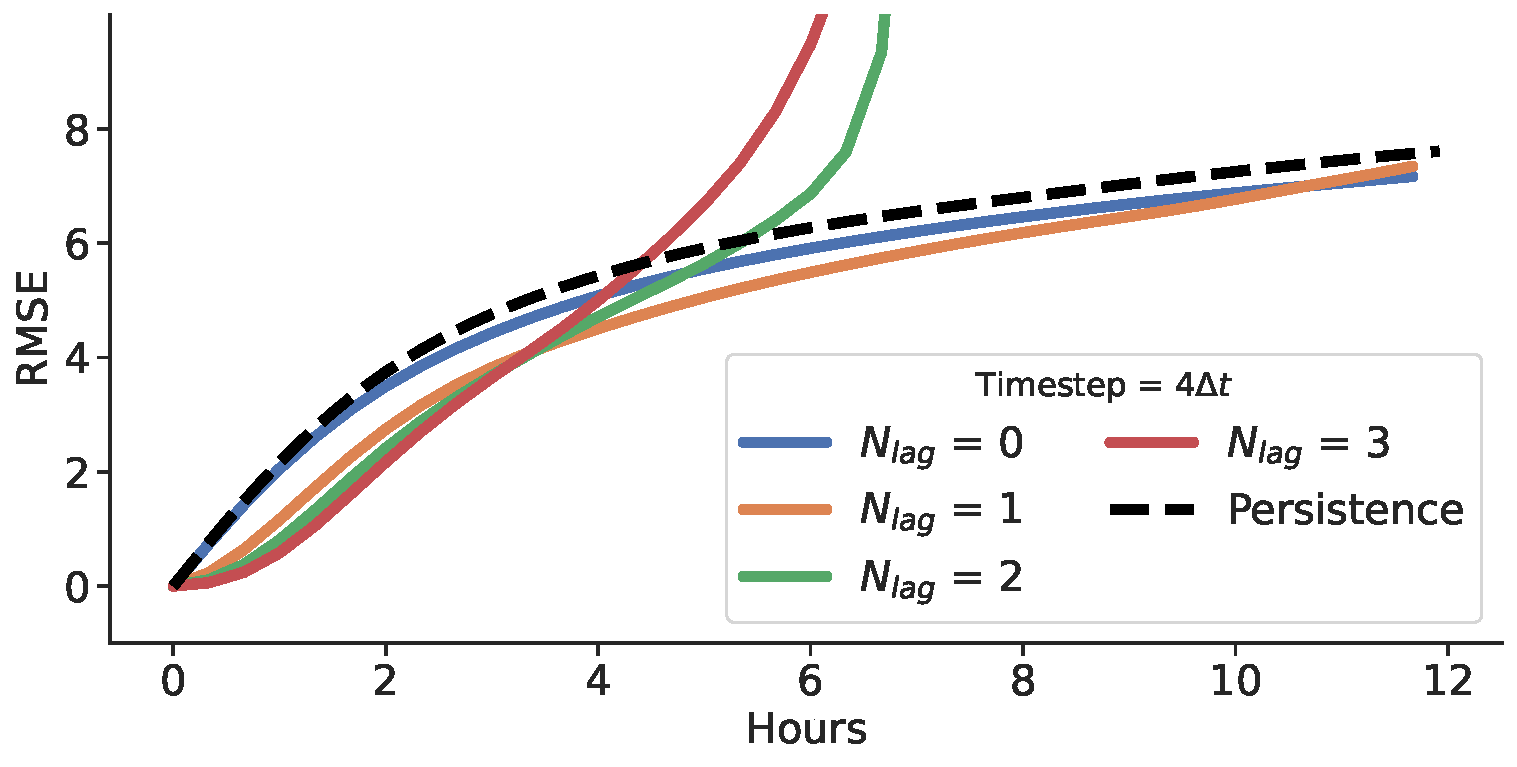
\includegraphics[width=.49\textwidth,
            trim={0, -2em, 0, 0}, clip]{../../figures/nvar-rmse-vs-lag-04sub.pdf}
        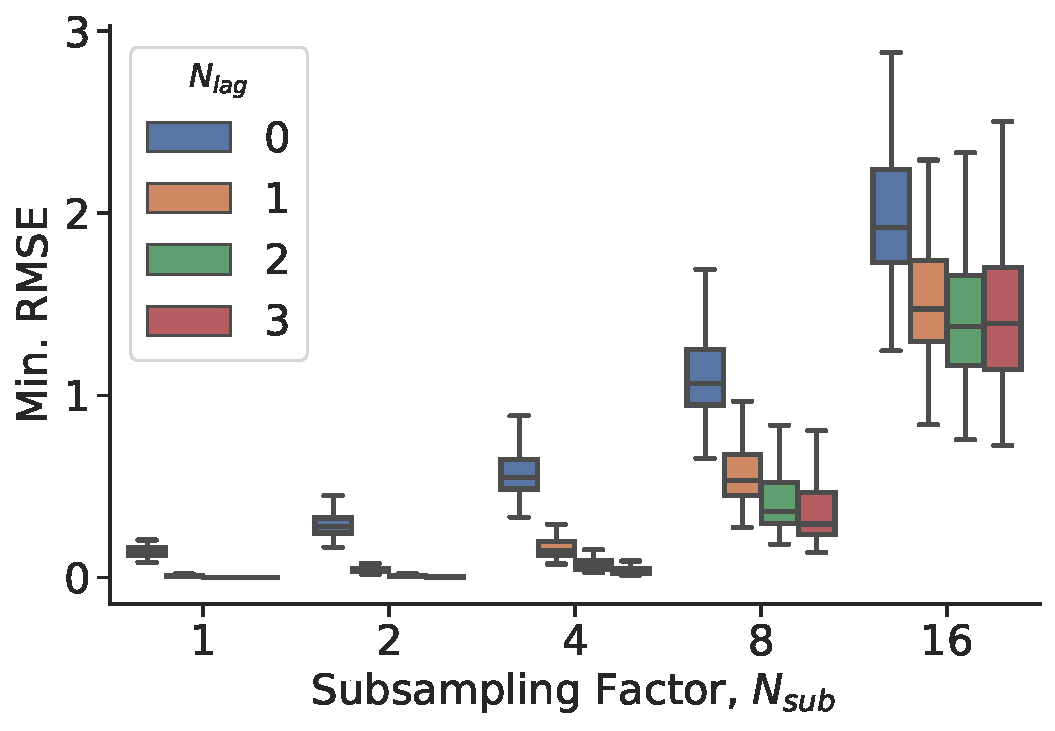
\includegraphics[width=.49\textwidth]{../../figures/nvar-mrmse-vs-lag-050samples.pdf}
    \end{minipage}

    \vspace{1.5em}
    \begin{minipage}{\textwidth}
        \begin{itemize}
            \item Increasing memory improves prediction skill, with diminishing returns
            \item For $n<=4$, prediction skill
                approaches that of RNN trained on model timestep
            \item Quadratic NVAR does not capture nonlinear
                interactions between time-lagged states
            \item Corroborates \cite{zhang_catch-22_2022}: small
                uncertainties and\\inaccuracies in NVAR nonlinearity are
                detrimental to prediction skill
        \end{itemize}
    \end{minipage}
\end{tcolorbox}
